\documentclass[a4paper, 11pt]{article}

% For figures
\usepackage{graphicx}
\DeclareGraphicsExtensions{.pdf,.png,.jpg}
\usepackage{float}

\usepackage[colorlinks]{hyperref}

% Initializing the counters and define a custom label
\newcommand{\reqinit}{
    % Create a new counter for keeping track of the last number
    \newcounter{reqcountbackup}
    % Create a new counter for the custom label
    \newcounter{reqcount}
    % Redefine the command for the last counter so when it is called
    % it prints the number like this in a bold font: R<number>
    \renewcommand{\thereqcount}{\textbf{R\arabic{reqcount}}}
}

% Used to define the start of the requirements
\newcommand{\reqstart}{
    % Indicate the start of a new list and tell it to use the redefined
    % command and corresponding counter for every item
    \begin{list}{\thereqcount}{\usecounter{reqcount}}
    % Important part: set the value of the used counter to the
    % same value of the backup counter.
    \setcounter{reqcount}{\value{reqcountbackup}}
}

% Used to define the end of the requirements
\newcommand{\reqend}{
    % Important part: take the value of the used counter (after
    % being incremented by the requirement items) and store it
    % in the backup counter.
    \setcounter{reqcountbackup}{\value{reqcount}}
    % Mark the end of the list environment
    \end{list}
}

\title{Accessible Pointing Approaches for Web Applications -- Requirements Specification \& Design}
\author{Alexander Birch}
\date{January 2014}

\begin{document}
\maketitle
\tableofcontents
\pagebreak

\reqinit

\section{Specification}
Here we capture the main engineering goals of the software system to be produced. An attempt is made to refrain from prescribing a specific implementation.

\newcommand{\reqitem}[2]{\item {#1} \\\textit{#2}}

\subsection{Non-functional requirements}

These requirements have a high priority:
\reqstart
    \reqitem{High availability}{Neither price nor platform should be a barrier to adoption of the software. A solution that works in many browsers would be most available.}
    \reqitem{Good citizenship (input)}{Bindings reserved for interaction with software should not conflict with those required by web browser, or (within reason) bindings that webpage will use.}
    \reqitem{Good citizenship (output)}{Interface displayed by software should not prevent reading of webpage.}
    \reqitem{Predictability}{User should be able to anticipate the outcome of their actions in advance.}
    \reqitem{Intuitivity (output)}{User should be able to understand the output of the system.}
    \reqitem{Intuitivity (input)}{User should be able to understand what to input into the system.}
    \reqitem{No time constraints}{There should exist no time-sensitive interactions; user might be disabled in a way that makes it difficult to input quickly.}
    \reqitem{Independent of markup}{It is wishful to expect all visited websites to have sane markup, so semantics should not be relied upon. We point at the things that we can see, so a pointing system should be based around the visual layout of the page, rather than the semantics.}
    \reqitem{Resilient to change}{Many modern websites have changing interfaces, such as content being loaded in dynamically, or elements changing state (ie collapsible components).}
    %\reqitem{}{}
\reqend

Some of these requirements are inherently at odds with the choice to use a web extension hosted within the content of the page under navigation; necessarily, the interface of the software displayed in the webpage will need to overlap content on said webpage, and there is no telling in advance which keybindings will cause conflicts with an unknown webpage. The hope is that a solution can be found that works with a usefully large portion of the Web.

These requirements have a low priority:
\reqstart
    \reqitem{Co-citizenship with tabbing}{Existing tabbing navigation should still be available to user, as it is still useful for some tasks (e.g. form navigation).}
\reqend

\subsection{Non-functional requirements}


These requirements have a high priority:
\reqstart
	\reqitem{Efficient navigation (semantically unrelated elements)}{Navigation to elements that exist in separate visual containers to the currently focused element, should be possible in less than 4 keypresses.}
	\reqitem{Efficient navigation (semantically related, but distant elements)}{Navigation to elements that exist in the same visual container as the currently focused element, should be possible in less than 4 keypresses.}
	\reqitem{Efficient navigation (arbitrary position)}{Navigation to elements that exist in the same visual container as the currently focused element, should be possible in less than 4 lookups.}
    %\reqitem{}{}
\reqend

\subsection{Anti-requirements}

The following are explicitly \textit{not} aims of the system, so performance in these areas need not be measured.

\reqstart
	\reqitem{Efficient navigation (semantically related, nearby elements)}{Navigation to elements that exist in the same visual container as the currently focused element, and are nearby: tabbing navigation already performs this very efficiently (albeit unpredictably). The more pressing concern is how to navigate between visual containers.}
	\reqitem{Navigation to off-screen elements}{In this pointing-based interface, it is assumed that the user will only ever be trying to navigate to elements that they can point at; thus off-screen elements need not be captured.}
	\reqitem{Fast navigation}{The goal is `efficient' navigation, not `fast' navigation. There can exist a correlation (less inputs will, from a GOMS perspectively, necessarily reduce task time also, provided cognitive and perceptual factors are negligible). But efficiency is the more important battle, as the system is targeted at low-bandwidth users, such as those with RSI (who need to avoid repetitive motor activity).}
	\reqitem{Better performance than mouse pointing}{This keyboard pointing method should be compared primarily to other keyboard pointing methods (ie tabbing navigation). It is for users who cannot use a mouse to point, i.e. due to physical reasons like disability, or interface constraints such as using a Smart TV Web browser requiring remote control input.}
    %\reqitem{}{}
\reqend

\pagebreak

\section{Design}
\subsection{Problem domain}
%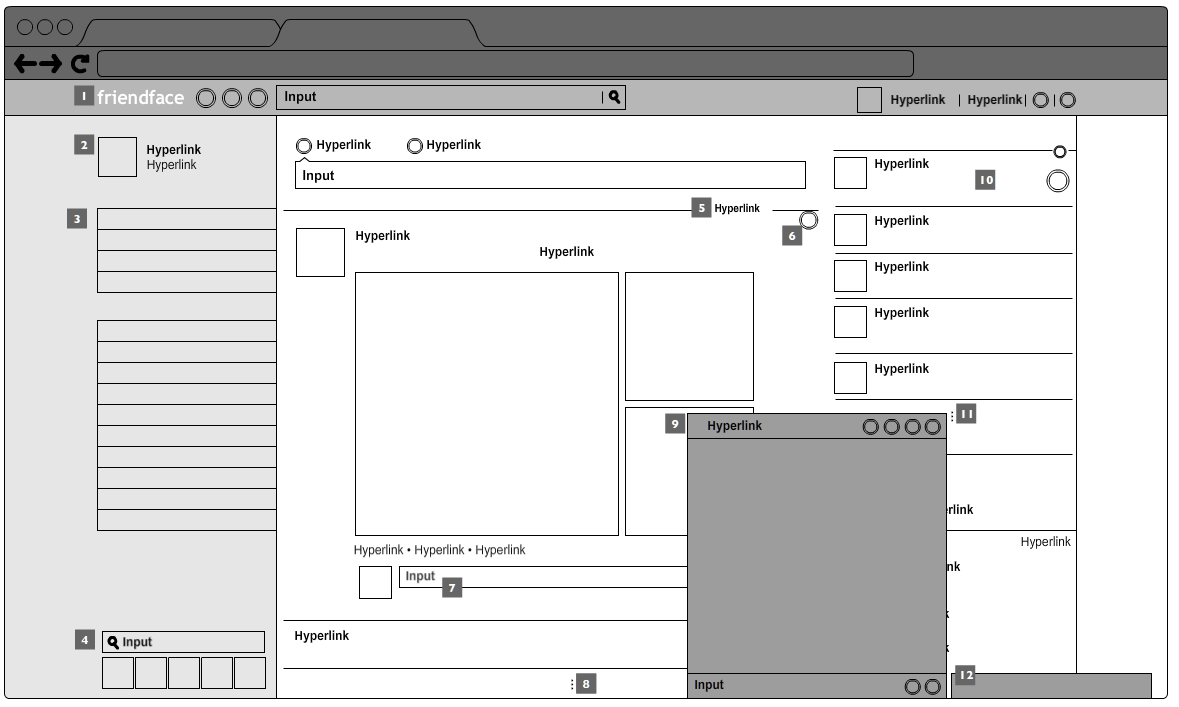
\includegraphics[width=\textwidth]{LowFidelityFacebookLabelled}

%\begin{figure}[H]
%\hspace*{-1.5in}
%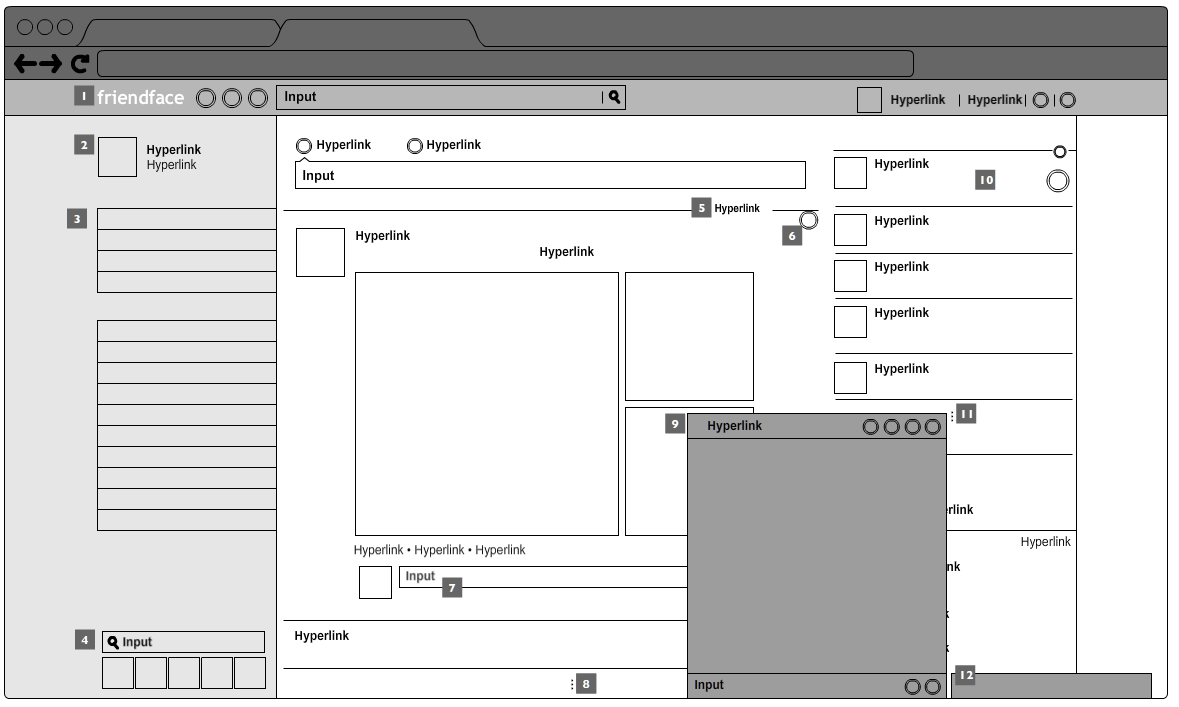
\includegraphics[width=8in]{LowFidelityFacebookLabelled}
%\end{figure}

\begin{figure}[H]
\centerline{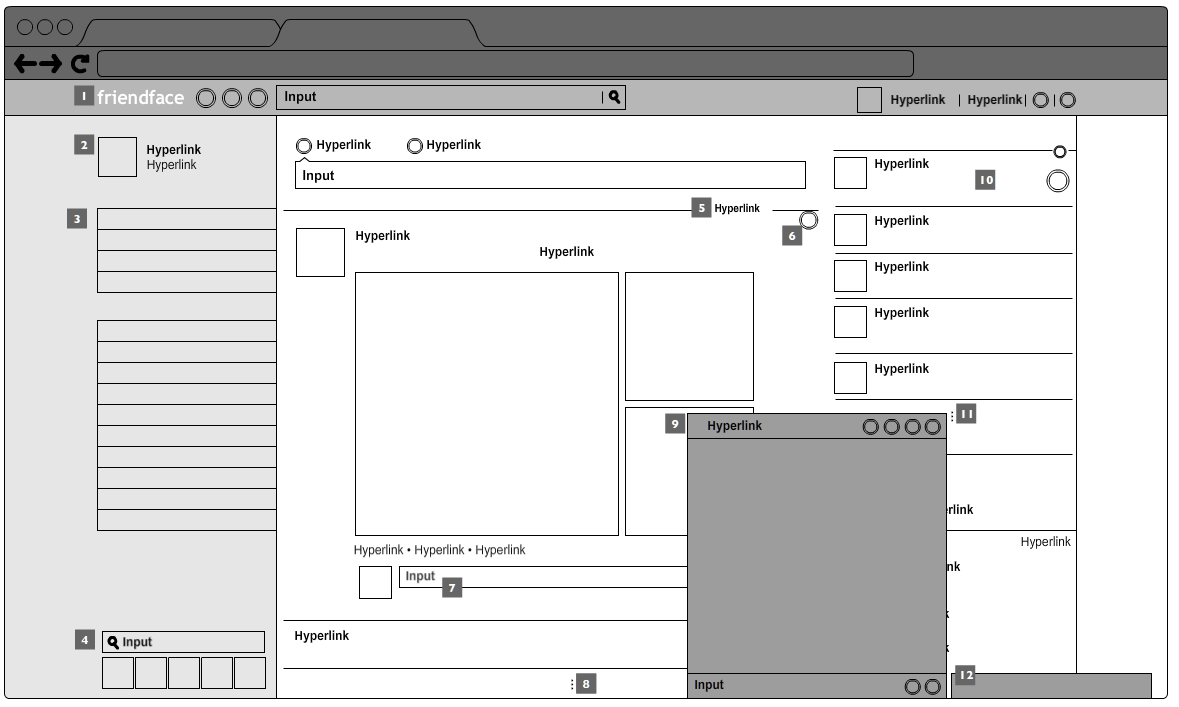
\includegraphics[width=8in]{LowFidelityFacebookLabelled}}
\caption{A typical complex web application layout.}
\label{fig:typicalWebAppLayout}
\end{figure}

 Our software solution will need to cope with the many and varied pointing scenarios presented in typical web applications like Figure ~\ref{fig:typicalWebAppLayout}. Some discrete cases of interest have been labelled; a discussion follows, regarding what is significant about these cases, and how we could consider optimizing our software for such cases.


\newcounter{problemdomainfigcount}

\newcommand{\someprob}[2]{\stepcounter{problemdomainfigcount}\indent\textbf{\arabic{problemdomainfigcount} #1}\\\noindent#2\\}

\someprob{Navigation bar floats above content}{This is a `web application' version of interface `chrome' (application controls around the content). Intuitive pointing needs to respect the current visual position of the content, and understand that the content can scroll under the floating chrome. Tab navigation ignores the presented position of the content, and can focus off-screen elements (despite the user's not being able to see such elements). It would be more efficient to restrict the search space to visible, on-screen elements (i.e. things that can be `pointed' at).}
\someprob{Elements can duplicate each other's actions}{For example, a hyperlink could be the caption to some icon, and clicking either would produce the same result. In a poorly-marked-up page, a tab journey would traverse both of these elements, despite their function being equivalent. A more efficient mechanism would be one that allows the user to skip past duplicates (by combining them conceptually into one control, or otherwise by allowing the user to jump over multiple elements in a traversal).}
\someprob{Repeating units of repeating units}{These sets of buttons are grouped into categories. If the user can express that they are interested in a category, it could eliminate other categories entirely from the search space. Similarly, if repeating units could be detected, then an explicit list traversal mechanism could be offered to the user. Detection of such things is likely to be difficult though, as it requires sane markup.}
\someprob{Unskippable lists}{Similar to the previous point, a list of elements can be marked up without the use of an explicit list component (for example, a drop-down). In tab-navigation, skipping past the list is impossible; the user must tab past each individual element. A better traversal method would not rely on explicit list markup for entering and escaping lists.}
\someprob{Rarely-used elements}{Though it needs to be possible to point at all elements, it is not ideal for obscure elements to appear in the majority of tab journeys (the user only wants to traverse them in exceptional cases). Our system needs to give the user control over the journey they take to point at an element, such that they can decide whether to traverse toward elements they would otherwise avoid.}
\someprob{Invisible elements}{Some elements only present themselves upon mouseover or keyboard focus. Similarly, components like menus might expand as an option is touched on mouseover. Our pointing system might need to provide the user with an equivalent mechanism to `mouseover' to probe for invisible elements. In particular, actions other than `click' should be made available for interacting with the environment.}
\someprob{Many forms}{A page can contain many small forms that are unrelated to each other. Since tab navigation is relatively good at traversing forms, browsers like Safari allow the user to traverse just form components. But it is hard to be sure whether pressing tab will move to the next element in some form, or to a different form altogether. It needs to be clear to the user how far they will move when they interact, so a visual indicator of the constraints of the search would be useful.}
\someprob{Infinite Scrolling}{Many websites with dynamic content recruit `infinite scrollers' to procedurally load in more content as the user scrolls the page. These are dangerous to tab navigation, which traverses depth-first; once it is in an infinite feed, it cannot escape, since as focus approaches the `end' of the content, further content is loaded indefinitely. Thus elements after an infinite content feed are rendered unreachable. This is another case where our traversal system will absolutely need to provide a skipping mechanism, or choice of route.}
\someprob{Layout Occlusion}{Floating elements can occlude those elements behind them. Thus it becomes impossible to point at the occluded elements. Actually, tab navigation copes very well with this problem (as it traverses by markup, rather than visual position). Our system will not try to solve this problem though, since even mouse pointing suffers from this. Since websites are mouse-optimized, it is expected that they would avoid creating problematic occlusion scenarios, or at least make them reversible (for example, some occluding content can be collapsed).}
\someprob{Repeated units of varying size}{Identification of repeating units based on a visual analysis might be difficult, as the visual difference can be non-trivial; some elements can be larger than others. At any rate, our system will not attempt anything as complex as computer vision for understanding page layout. Ideally the system should be designed to not need an understanding of the page layout (like mouse navigation, which simply points at coordinates specified by the user).}
\someprob{Multiple Infinite Scrollers}{A page can recruit infinite scrollers for content other than just the main feed. Thus assumptions like `any infinite scrolled content is likely to be the main focus of the page' can't be so easily made. The main takeaway here is that our system should not optimize interaction based on some imagined understanding of the purpose of the page structure; it could easily make incorrect assertions, thus would not be resilient to bad or obscure web design.}
\someprob{Multi-modal Elements}{Elements can change size or state, for example collapsible components. Any representation the system stores about the layout of the webpage should be sensitive to this possibility of change.}
%\someprob{}{}

\end{document}